\documentclass[border=8pt]{standalone}
\usepackage{amssymb}
\usepackage{bbm}
\usepackage{fontspec}
\setmainfont{Source Serif 4}
\usepackage{pgfplots}
\pgfplotsset{compat=1.18}
\definecolor{qbase}{RGB}{31,86,160}
\definecolor{winner}{RGB}{209,73,91}

\begin{document}
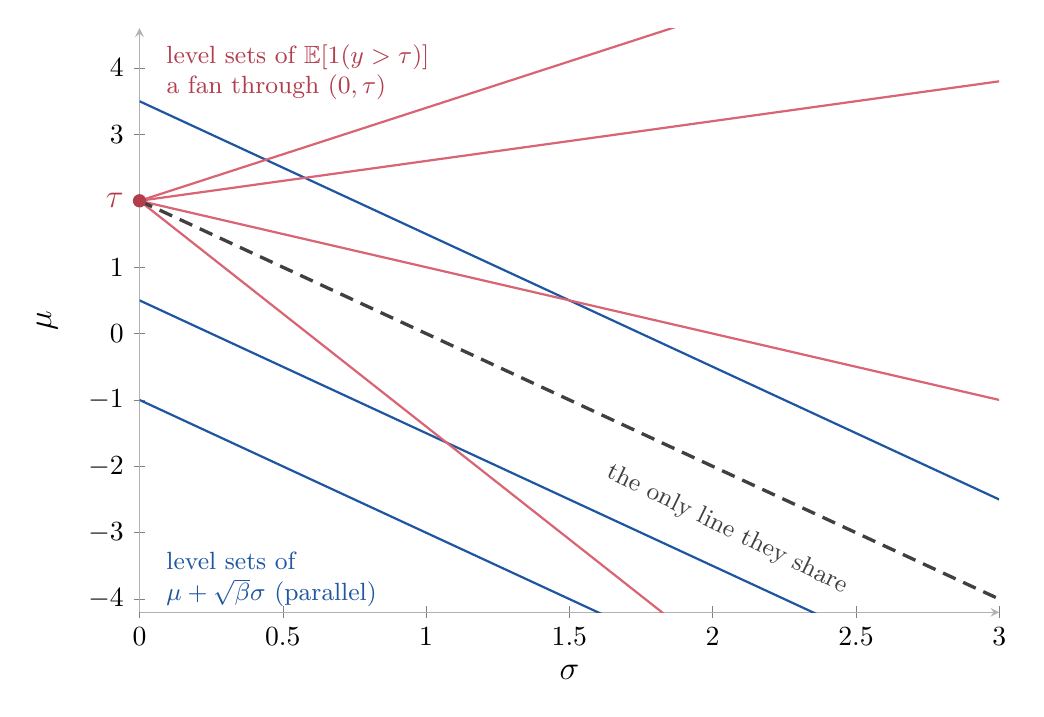
\begin{tikzpicture}
\begin{axis}[
  width=12.5cm, height=9cm,
  axis lines=left,
  xlabel={$\sigma$}, ylabel={$\mu$},
  xmin=0, xmax=3, ymin=-4.2, ymax=4.6,
  label style={font=\large},
  tick label style={font=\normalsize},
  axis line style={gray!60},
  ytick={-4,-3,-2,-1,0,1,3,4},
  extra y ticks={2},
  extra y tick labels={$\tau$},
  extra y tick style={tick label style={font=\large, winner!85!black}},
  clip=true,
]
% UCB level sets: mu = s - 2*sigma (parallel, slope -2)
\addplot[domain=0:3, samples=2, thick, qbase] {-1 - 2*x};
\addplot[domain=0:3, samples=2, thick, qbase] {0.5 - 2*x};
\addplot[domain=0:3, samples=2, thick, qbase] {3.5 - 2*x};
% PI(tau=2) level sets: mu = 2 + c*sigma (fan through (0,2))
\addplot[domain=0:3, samples=2, thick, winner!85] {2 - 3.4*x};
\addplot[domain=0:3, samples=2, thick, winner!85] {2 - 1*x};
\addplot[domain=0:3, samples=2, thick, winner!85] {2 + 0.6*x};
\addplot[domain=0:3, samples=2, thick, winner!85] {2 + 1.4*x};
% the one shared line: c = -2 coincides with s = 2
\addplot[domain=0:3, samples=2, very thick, dash pattern=on 5pt off 3pt, black!75] {2 - 2*x};
% fan apex
\addplot[only marks, mark=*, mark size=2.2pt, winner!85!black] coordinates {(0,2)};
% labels, placed in line-free regions
\node[winner!85!black, font=\small, anchor=north west, align=left] at (axis cs:0.06,4.5)
  {level sets of $\mathbb{E}[\mathbbm{1}(y > \tau)]$\\ a fan through $(0, \tau)$};
\node[qbase, font=\small, anchor=north west, align=left] at (axis cs:0.06,-3.15)
  {level sets of\\ $\mu + \sqrt{\beta}\sigma$ (parallel)};
\node[black!75, font=\small, anchor=center, rotate=-26] at (axis cs:2.05,-2.95)
  {the only line they share};
\end{axis}
\end{tikzpicture}
\end{document}
